
\documentclass{ximera}
%% handout
%% nohints
%% space
%% newpage
%% numbers

%% You can put user macros here
%% However, you cannot make new environments

\graphicspath{{./}{firstExample/}{secondExample/}}

\usepackage{url}
\usepackage{tikz}
\usepackage{tkz-euclide}
\usetkzobj{all}


\tikzstyle geometryDiagrams=[ultra thick,color=blue!50!black]
\pgfplotsset{compat=1.8}
  \usepackage[T1]{fontenc}
  \usepackage[utf8x]{inputenc}


\prerequisites{none}

\title{Conditional Probability}

\begin{document}
\begin{abstract}
We introduce the idea of conditional probability and work through some simple examples.
\end{abstract}
\maketitle

\subsection*{Basic learning objectives}

These are the tasks you should be able to perform with reasonable fluency \textbf{when you arrive at our next class meeting}. Important new vocabulary words are indicated \emph{in italics}. 

\begin{itemize}
    \item Understand the definition of a \emph{conditional probability} and its relationship to the general concept of probability.
    \item Be able to compute a conditional probability by counting objects in a sample space.
\end{itemize}

\subsection*{Advanced learning objectives}

In addition to mastering the basic objectives, here are the tasks you should be able to perform \textbf{after class, with practice}: 

\begin{itemize}
    \item Compute conditional probabilities using a probability tree.
    \item Apply the concept of conditional probability to the example of the \emph{false positive paradox}.
\end{itemize}

\noindent\hrulefill

When working with probabilities, we sometimes want to make certain types of restrictions to our sample space. For example, asking what the probability is that a person will make a 3-point basketball shot is different than asking what the probability is that a professional basketball player will make a 3-point shot. The restriction that the person is a professioinal basketball player restricts the sample space. This could be phrased as, ``What is the probabilith that a person will make a 3-point shot \emph{given that} the person is a professional basketball player?''

Restricting the sample space can sometimes lead to interesting situations that are not intuitive. A \emph{conditional probability} is a probability with a restriction on the sample space. The notation for conditional probabilities is the following:
$ P(X | Y) =$ ``The probability that event $X$ occurs given that event $Y$ occurred.''

In the case that all events are equiprobable, we can use a formula that is similar to the one we used for basic probabilities (which we will repeat here for reference).
\begin{align*}
  P(X) & = \dfrac{ \# \text{ of successes (for $X$)}}{ \# \text{ of possibilities } } \\ \\
  P(X | Y) & = \dfrac{ \# \text{ of successes for $X$ where $Y$ also happens}}{ \# \text{ of possibilities where $Y$ happens}}
\end{align*}

The best way to understand these situations is to think through a couple examples. Suppose that you are doing an experiment of rolling two standard 6-sided dice. The sample space contains 36 elements:
\begin{image}
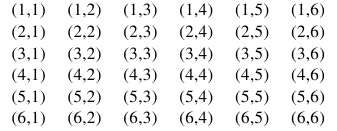
\includegraphics{ConditionalProbTable1.png}
%\begin{tabular}{cccccc}
%    (1,1) & (1,2) & (1,3) & (1,4) & (1,5) & (1,6) \\
%    (2,1) & (2,2) & (2,3) & (2,4) & (2,5) & (2,6) \\
%    (3,1) & (3,2) & (3,3) & (3,4) & (3,5) & (3,6) \\
%    (4,1) & (4,2) & (4,3) & (4,4) & (4,5) & (4,6) \\
%    (5,1) & (5,2) & (5,3) & (5,4) & (5,5) & (5,6) \\
%    (6,1) & (6,2) & (6,3) & (6,4) & (6,5) & (6,6) \\
%\end{tabular}
\end{image}

What is the probability of rolling a 3 given that the total is 6 or greater? Notice that our successes ($X$) are described by rolling a 3, but the extra condition ($Y$) is that the total is 6 or greater.

The first task is to restrict the sample space to combinations that add up to 6 or greater. We will indicate the rejected outcomes being by blacking them out in the table below:
\begin{image}
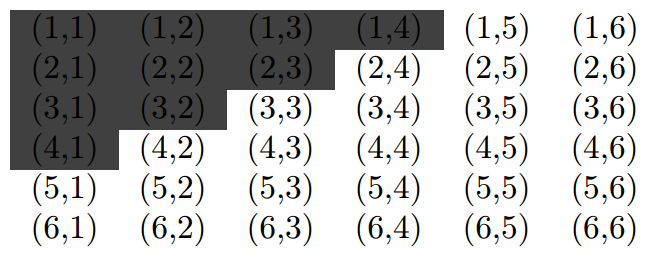
\includegraphics{ConditionalProbTable2.png}
%\begin{tabular}{cccccc}
%    \cellcolor{darkgray}(1,1) & \cellcolor{darkgray}(1,2) & \cellcolor{darkgray}(1,3) & \cellcolor{darkgray}(1,4) & (1,5) & (1,6) \\
%    \cellcolor{darkgray}(2,1) & \cellcolor{darkgray}(2,2) & \cellcolor{darkgray}(2,3) & (2,4) & (2,5) & (2,6) \\
%    \cellcolor{darkgray}(3,1) & \cellcolor{darkgray}(3,2) & (3,3) & (3,4) & (3,5) & (3,6) \\
%    \cellcolor{darkgray}(4,1) & (4,2) & (4,3) & (4,4) & (4,5) & (4,6) \\
%    (5,1) & (5,2) & (5,3) & (5,4) & (5,5) & (5,6) \\
%    (6,1) & (6,2) & (6,3) & (6,4) & (6,5) & (6,6) \\
%\end{tabular}
\end{image}
We will remove the blackened combinations because we are not interested in them at all. Within the remaining sample space, we need to count the events that have a 3 in them:
\begin{image}
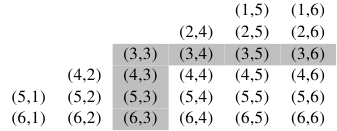
\includegraphics{ConditionalProbTable3.png}
%\begin{tabular}{cccccc}
%     &  &  &  & (1,5) & (1,6) \\
%     &  &  & (2,4) & (2,5) & (2,6) \\
%     &  & \cellcolor{lightgray}(3,3) & \cellcolor{lightgray}(3,4) & \cellcolor{lightgray}(3,5) & \cellcolor{lightgray}(3,6) \\
%     & (4,2) & \cellcolor{lightgray}(4,3) & (4,4) & (4,5) & (4,6) \\
%    (5,1) & (5,2) & \cellcolor{lightgray}(5,3) & (5,4) & (5,5) & (5,6) \\
%    (6,1) & (6,2) & \cellcolor{lightgray}(6,3) & (6,4) & (6,5) & (6,6) \\
%\end{tabular}
\end{image}
We can see that there are 7 combinations that contain a 3 and a total of 26 combinations that met the condition. This means that the probability is $\frac{7}{26} \approx 26.9\%$. (For comparison, the probability of rolling a 3 when rolling two dice without the restriction is $\frac{11}{36} \approx 30.6\%$.)

This may not seem that complicated, but the next video will show some highly non-intuitive results that happen with conditional probabilities. Consider the following question: A man has two children. At least one of those children is a boy. What is the probability that the other child is also a boy? (Think for a moment!)

You probably guessed 50\%. And you would be wrong. Knowing that one of the children is a boy actually \emph{reduces} the chances of the second child being a boy. Almost everybody is tricked by this problem.

This is known as the boy-boy paradox (or sometimes the boy-girl paradox, if the question is asking for the probability that the other child is a girl). The following video will explain the paradox and give you more experience with conditional probabilities: \youtube{https://www.youtube.com/watch?v=RA6POO0x9h8}.

\begin{question}
What does $P(X|Y)$ mean?

    \begin{multipleChoice}
      \choice{The probability that events $X$ and $Y$ both happen.}
      \choice[correct]{The probability that event $X$ happened, given that event $Y$ has also happened.}
      \choice{The probability that event $Y$ happened, given that event $X$ has also happened.}
      \choice{The probability that event $Y$ happened, but event $X$ didn't happen.}
    \end{multipleChoice}

\end{question}

\begin{question}
When rolling two dice, determine the probability of rolling a 1 given that the total is 6 or greater.

    \begin{multipleChoice}
      \choice{$\frac{11}{36}$}
      \choice{$\frac{1}{6}$}
      \choice[correct]{$\dfrac{2}{13}$}
      \choice{$\frac{1}{3}$}
    \end{multipleChoice}
    \begin{hint}
      Use the restricted sample space from the example that is similar to this one.
    \end{hint}

\end{question}

\begin{question}
A man has two children. At least one of those children is a boy. What is the probability that the other child is also a boy?

    \begin{multipleChoice}
      \choice[correct]{$\dfrac{1}{3}$}
      \choice{$\dfrac{1}{2}$}
      \choice{$\dfrac{2}{3}$}
    \end{multipleChoice}

\end{question}


\end{document}